\chapter{Background}
\label{chap:background}

In this chapter, I introduce the biological concepts and methods that will be used throughout this manuscript.
I first present DNA supercoiling and its regulation in bacteria.
I outline its role in gene transcription, and the converse effect of transcription on supercoiling, which jointly result in the so-called transcription-supercoiling coupling.
Then, I discuss a few cases studies in which supercoiling might have played an important evolutionary role, and that epitomize the interest of the study of supercoiling under an evolutionary light.
Finally, I present the general method with which I tackle the questions raised in Chapter~\ref{chap:intro} throughout the manuscript.

\section{DNA Supercoiling in Bacteria}
\label{sec:background:sc}

\begin{figure}
  \centering
  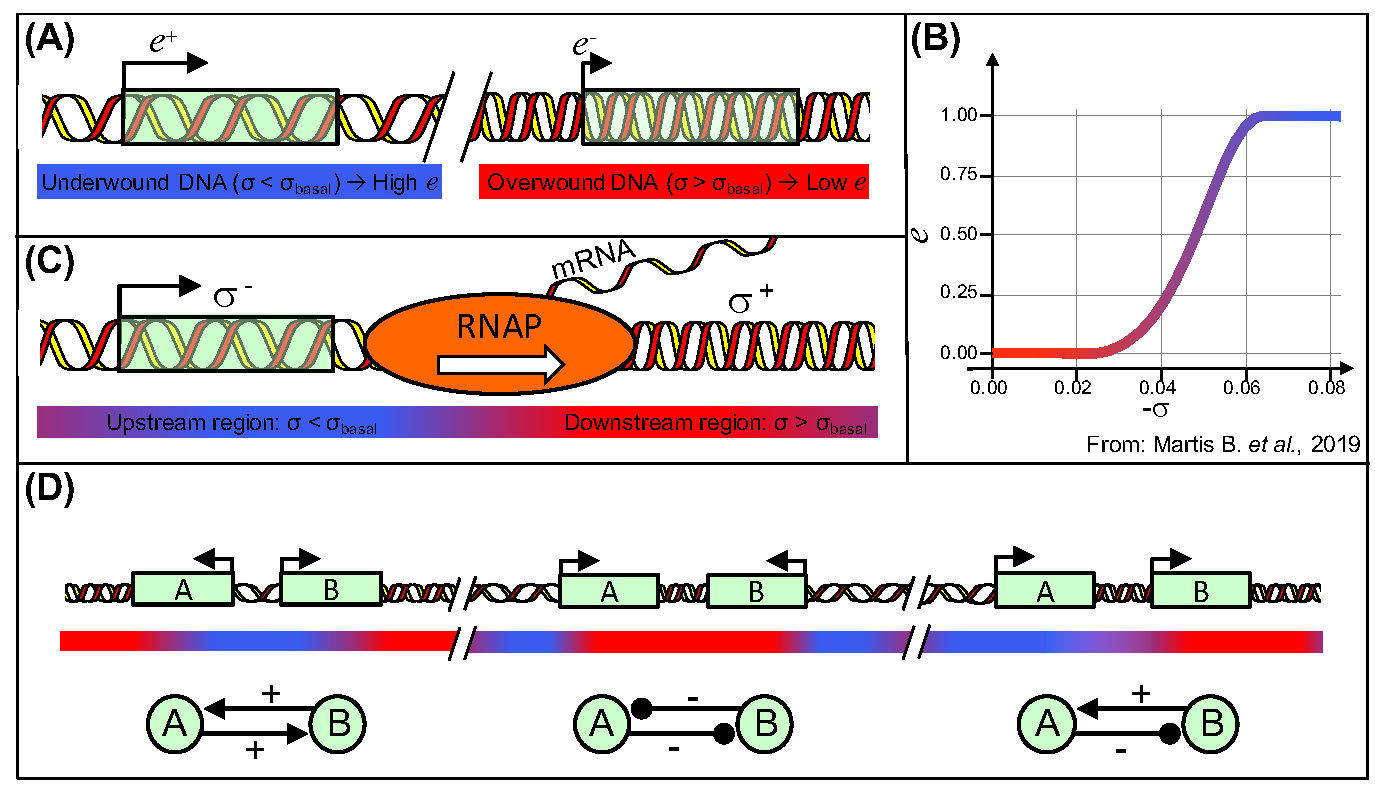
\includegraphics[width=\textwidth]{alife/img/fig-theorique.pdf}
  \caption[Role of supercoiling in transcription, and description of the TSC]{\textbf{A}. When DNA is underwound ($\sigma < \sigma_{basal}$, left), gene transcription rates are higher than when DNA is overwound ($\sigma > \sigma_{basal}$, right).
  \textbf{B}. Promoter activity (equivalently, transcription level) \emph{e} increases with the level of negative supercoiling $-\sigma$.
  \textbf{C}. The transcription of a gene by RNA polymerase (RNAP) generates a decrease in supercoiling upstream of the transcribed gene, and an increase downstream of the transcribed gene.
  \textbf{D}. Transcription-supercoiling coupling: the sign of the interaction between neighboring genes depends on their relative orientation.}
  \label{fig:background:theory}
\end{figure}

%\paragraph{Definition of DNA supercoiling}
DNA is the material basis of genetic information.
It is a flexible polymer that comprises two strands of nucleotides that coil around each other, at a rate of 10.5 base pairs per turn.
When subjected to torsional stress, DNA can either writhe and form 3-dimensional loops, or twist around itself more or less tightly than in its relaxed state~\citep{travers2005}; both writhing and twisting are referred to as DNA supercoiling.
The level of supercoiling is measured as the relative density $\sigma$ of supercoils in over- or under-wound DNA, as compared to relaxed DNA.
DNA is positively supercoiled ($\sigma > 0$) when it is overwound, and negatively supercoiled ($\sigma < 0$) when it is underwound.
In bacteria, DNA is normally maintained in a moderately negatively supercoiled state, with a reference value of $\sigma_{basal}=-0.06$ in \emph{Escherichia coli}~\citep{travers2005}.

%\paragraph{Regulation of DNA supercoiling}
The level of DNA supercoiling in bacteria is controlled by topoisomerases, enzymes that alter DNA supercoiling by cutting and rotating the DNA strands~\citep{duprey2021}.
The two main topoisomerases are gyrase, which dissipates positive supercoiling by introducing negative supercoils at an ATP-dependent rate, and topoisomerase I, which oppositely relaxes negative supercoiling~\citep{martisb.2019}.
Many other processes additionally influence the level of DNA supercoiling.
While the intrinsic flexibility of the DNA polymer would in principle allow supercoils to propagate freely along its length, many nucleoid-associated proteins such as FIS, H-NS or HU bind to bacterial DNA~\citep{krogh2018}, in addition to RNA polymerases during gene transcription.
These nucleoid-associated proteins create barriers that block in practice the diffusion of supercoils, resulting in what have been termed topological domains of supercoiling~\citep{postow2004}.
At a local scale, according to the twin-domain of supercoiling~\citep{liu1987}, the transcription of a gene by RNA polymerase generates positive and negative supercoils.
A buildup of positive supercoiling can be observed upstream of the gene, and of negative supercoiling downstream of the gene, as a consequence of the rotational drag that hampers the rotation of RNA polymerases around DNA as they transcribe~\citep{visser2022}.
This phenomenon is pictured in subfigure C of Figure~\ref{fig:background:theory}.
The level of DNA supercoiling can furthermore be affected by numerous environmental challenges in bacteria.
Salt shock transiently increases negative DNA supercoiling in \emph{E. coli}~\citep{hsieh1991}; the acidic intracellular environment relaxes DNA in the facultative pathogen \emph{Salmonella enterica} var. Typhimurium~\citep{marshall2000}; and higher temperatures relax DNA in the plant pathogen \emph{Dickeya dadantii}~\citep{herault2014}.
These constraints overall result in a very dynamic DNA ``supercoiling landscape'' in \emph{E. coli}~\citep{visser2022}, with a supercoiling level that varies in both time during the bacterial lifecycle and space along the chromosome.

%\paragraph{Effect of supercoiling on transcription}
The level of DNA supercoiling influences gene expression, as a more negatively supercoiled DNA facilitates the initiation of transcription by RNA polymerase~\citep{elhoudaigui2019}, as pictured in subfigures A and B of Figure~\ref{fig:background:theory}.
This general response has been shown to depend in particular on both promoter sequence~\citep{forquet2021} and spacer length~\citep{forquet2022}.
Many bacteria leverage this regulating effect of DNA supercoiling on gene transcription by modulating their DNA supercoiling level.
In several bacteria such as \emph{E. coli}, \emph{S. enterica}, or \emph{D. dadantii}, between 5\% and 15\% of genes were found to be sensitive to relaxation or hypercoiling of chromosomal DNA, with genes being up-regulated or down-regulated in each condition~\citep{peter2004, ferrandiz2010, webber2013, pineau2022a}.
DNA supercoiling might in particular be an especially important regulator of gene activity in bacteria with reduced genomes, such as the obligate aphid endosymbiotic bacterium \emph{Buchnera aphidicola}, which is nearly devoid of transcription factors~\citep{brinza2013}.

\section{The Transcription-Supercoiling Coupling}

As we saw above, the process of transcribing a given gene generates an accumulation of positive supercoiling downstream of that gene, and of negative supercoiling upstream of that gene~\citep{liu1987,visser2022} (Figure~\ref{fig:background:theory}C).
If a second gene is located closely enough to this first gene, the change in supercoiling at the promoter of the second gene will impact its transcription rate, as negative supercoiling usually facilitates promoter opening, and hence gene transcription~\citep{forquet2021}.
In turn, the transcription of the second gene will also generate a local change in supercoiling that affects the first gene, resulting in an interaction between the transcription levels of these two genes, which has been called the transcription-supercoiling coupling~\citep{meyer2014}.
Depending on the relative orientation of these genes, the coupling can take several forms.
Divergent genes increase their respective transcription level in a positive feedback loop; convergent genes inhibit the transcription of one another; and in tandem genes, the transcription of the downstream gene increases the transcription of the upstream gene, while the transcription of the upstream gene decreases the transcription of the downstream gene.

This supercoiling-mediated interaction between neighboring genes has been documented in several bacterial genetic systems.
In the \emph{E. coli}-related pathogen \emph{Shigella flexneri}, the \emph{virB} promoter is normally only active at high temperature, but can be activated at low temperature by the insertion of a phage promoter in divergent orientation~\citep{tobe1995}.
Similarly, the expression of the \emph{leu-500} promoter in \emph{S. enterica} can be increased or decreased by the insertion of upstream transcriptionally active promoters, depending on their orientation relative to \emph{leu-500}~\citep{elhanafi2000}.
The magnitude of the effect of the transcription-supercoiling coupling has also been explored in a synthetic construct, in which the inducible \emph{ilvY} and \emph{ilvC} \emph{E. coli} promoters have been inserted on a plasmid in divergent orientations.
In this system, a decrease in the activity of \emph{ilvY} is associated with a decrease in \emph{ilvC} activity, and an increase in \emph{ilvY} activity with an increase in \emph{ilvC} activity as well~\citep{rhee1999}.

There are, however, hints that the biological relevance of the transcription-supercoiling coupling might not be confined to a few specific cases.
Indeed, in \emph{E. coli}, the typical size of topological domains --  inside which the supercoiling generated by gene transcription can propagate -- usually stands around 10kb~\citep{postow2004}, transcription-generated supercoiling could propagate up to 25kb in each direction around a transcribed gene~\citep{visser2022}.
As the average size of \emph{E. coli} genes is 1kb, and the average intergenic distance about 120bp~\citep{blattner1997}, this means that any single topological domain can encompass multiple genes, which can potentially interact via the transcription-supercoiling coupling.
A statistical analysis of the relative position of neighboring genes on the \emph{E. coli} chromosome indeed shows that genes that are up-regulated by negative supercoiling have more neighbors in divergent orientations, while genes that are down-regulated by negative supercoiling have more neighbors in converging orientations~\citep{sobetzko2016}, suggesting that the transcription-supercoiling coupling plays a role in regulating the activity of these genes.

\section{Supercoiling and Evolution}

\subsection{LTEE}

Moreover, selection can act on the level of DNA supercoiling in order to modulate the regulation of gene expression.
In 10 of the 12 populations in the Long-Term Evolution Experiment (LTEE), an increase in fitness was linked to mutations in the \emph{topA} and \emph{fis} genes, which participate in the regulation of the supercoiling level~\citep{crozat2010}.
When inserted into the ancestral strain, these mutations increased the level of negative supercoiling as well as the bacterial growth rate~\citep{crozat2005}, demonstrating that the level of DNA supercoiling can evolve as part of a regulatory response to new environments.
In the Long-Term Evolution Experiment (LTEE)~\citep{lenski1991}, 12 populations of \emph{Escherichia coli} have been maintained for over 80,000 generations, evolving and adapting to a glucose-limited environment.
In this experiment, parallel increases in the level of negative supercoiling been measured in 10 of the populations~\citep{crozat2010}, suggesting that a more negatively supercoiled genome confers an evolutionary advantage for that environment.
Furthermore, mutations in two genes regulating DNA supercoiling, \emph{topA} and \emph{fis}, have been identified as the genetic basis for this phenotypic change, and have been verified to confer a fitness advantage~\citep{crozat2005} when inserted into the genetic background of the ancestral strain.
These results suggest a strong selection pressure to tune the level of DNA supercoiling to the new environment of the LTEE.

\subsection{Syntenies}
Finally, the regulation of gene expression by DNA supercoiling could be a force that participates in shaping the evolution of bacterial genomes themselves.
Indeed, supercoiling-sensitive genes tend to group in up or down-regulated clusters in \emph{E. coli}~\citep{peter2004}, \emph{S. enterica}~\citep{webber2013} and \emph{S. pneumoniae}~\citep{ferrandiz2010}, suggesting the possibility of an adaptive role in the co-localization of these clusters.
Indeed, synteny segments, or clusters of neighboring genes that show correlated expression patterns, are evolutionarily conserved across \emph{E. coli} and the distantly related \emph{Bacillus subtilis}~\citep{junier2016}, strengthening the hypothesis that these domains could play an important role in the regulation of bacterial gene expression.
\citep{sobetzko2016}!!

\subsection{Reduced genomes}
In addition to a localized influence, global gene regulation through changes in the DNA supercoiling level has been shown to exist in nature.
An example of this is \emph{Buchnera aphidicola}, an endosymbiotic bacteria with a streamlined genome, in which control of the supercoiling level has evolved to be one of the main regulatory mechanisms~\citep{brinza2013}.
Moreover, in \emph{Dickeya dadantii}, a plant pathogenic bacteria, different genomic regions exhibit markedly different responses to changes in supercoiling \citep{muskhelishvili2019}, allowing the expression of pathogenic genes only in stressful environments.
Finally, in the setting of experimental evolution, mutations in the regulation of supercoiling have been shown to drive the evolutionary response of \emph{Escherichia coli} strains.
In conclusion, DNA supercoiling plays an important evolutionary role.
It can serve as the support for the evolution of particular chromosomal organizations as a way to trigger certain sets of genes based on the change in supercoiling caused by specific environments, and its regulation is itself subject to selective pressure when adapting to new environments.

\section{Models of Supercoiling}

Several mathematical and computational models have been proposed to describe the effect of the transcription-supercoiling coupling on the expression level of neighboring genes.
In~\cite{meyer2014}, a quantitative model of the supercoiling level at a locus of interest is proposed.
DNA transcription is regulated by the opening energy of DNA around gene promoters, which directly depends on the supercoiling level.
In this model, the reciprocal influence of neighboring genes can be obtained by computing the difference in transcription levels due to supercoiling and the subsequent variation in supercoiling, and iterating this system until a fixed point is reached.
\cite{elhoudaigui2019} describe a more detailed stochastic model of DNA transcription involving explicit RNA polymerases and topoisomerases.
The transcription level of a genomic region of interest is simulated using discrete time steps, during which RNA polymerases attach to the DNA template, progress along the transcribed region while generating positive supercoiling downstream and negative supercoiling upstream, and detach from the DNA, relaxing supercoiling constraints.

These models however limit themselves to mechanistic descriptions of the local interaction between genes, but do not try to generalize to the whole-genome scale nor to an evolutionary time frame.

\section{Method: Evolutionary Systems Biology}

\begin{figure}
\centering
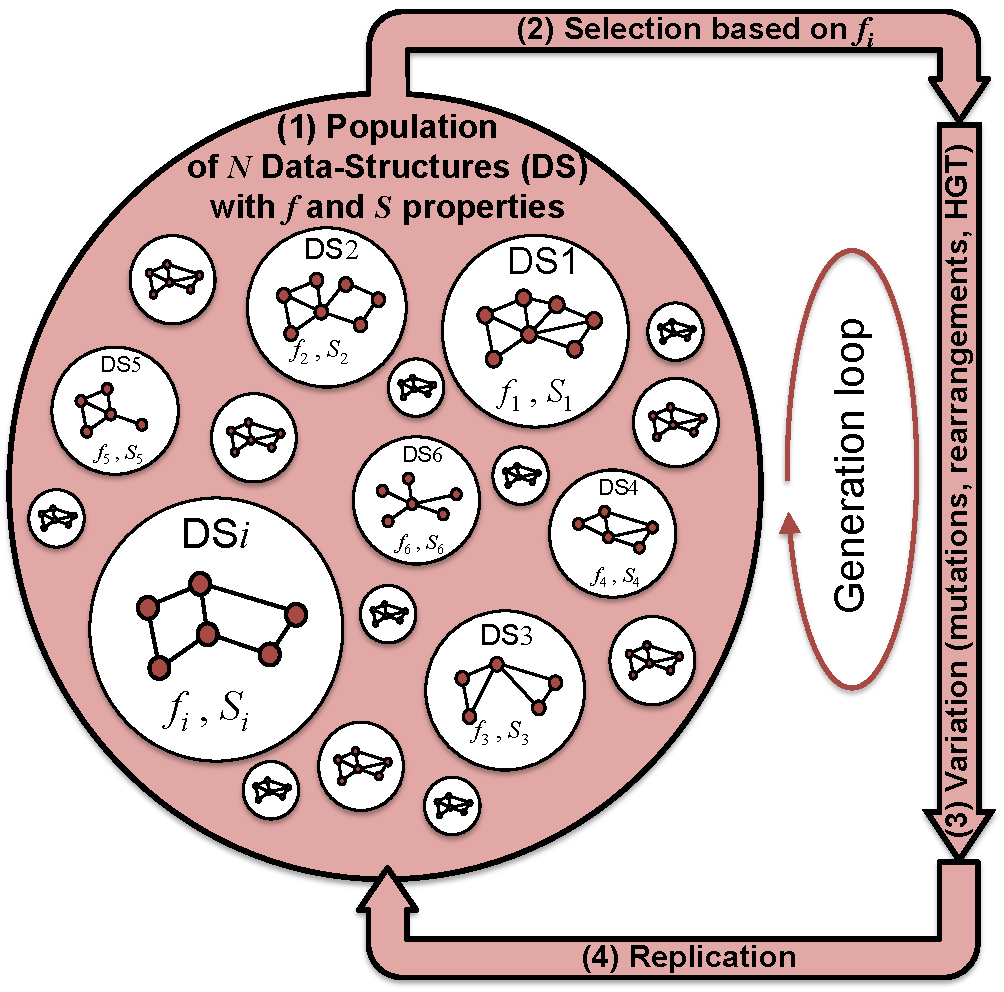
\includegraphics[width=0.9\textwidth]{background/img/evol_sys_bio.pdf}
\caption{A nice figure.}
\label{fig:background:evol-sys-bio}
\end{figure}

